% system_architecture.tex — Task 10 stub. Outline recovered verbatim from
% the original plan file fragment (see ../OUTLINE_NOTES.md). Draft at Task 12.
%
% Serverless stages ingestion -> extraction -> detection -> parsing ->
% validation -> persistence; prepare -> Step Functions Map -> merge
% batching; S3-as-bus intermediates. Note the batched production path
% differs from the direct path the evals use — say so (see
% tasking/arxiv_paper.md's batched-vs-direct background note).

\section{System Architecture}
\label{sec:system-architecture}

\begin{figure*}
  \centering
  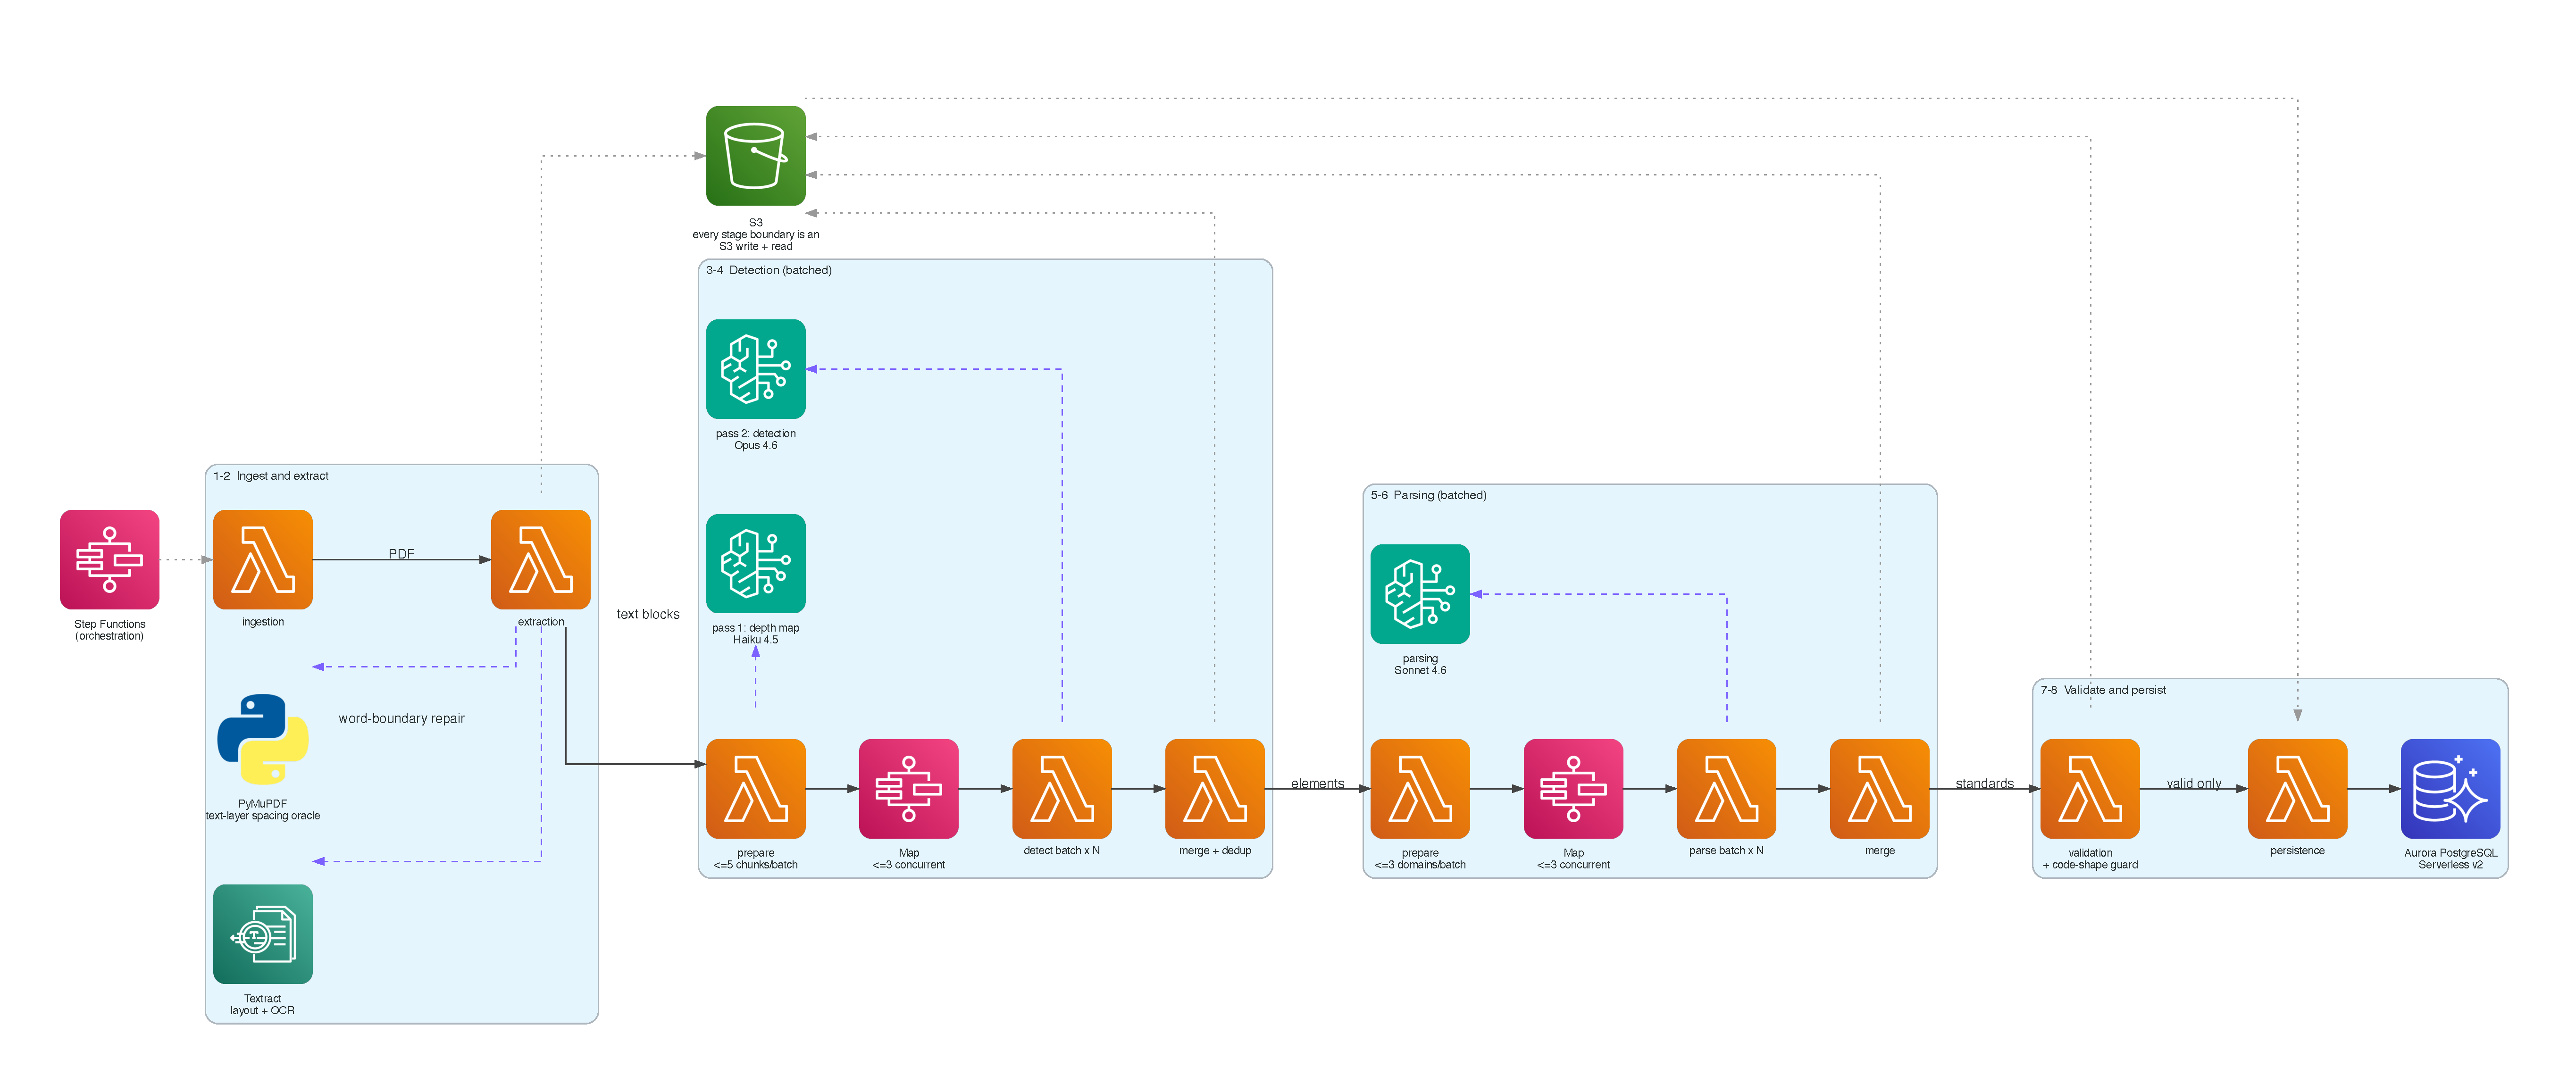
\includegraphics[width=\textwidth]{figures/fig_architecture.pdf}
  \caption{Pipeline architecture. Solid arrows carry data, dashed arrows are
  model calls, and dotted arrows mark JSON exchanged through S3. Regenerate with
  \texttt{python paper/analysis/make\_architecture\_figure.py}.}
  \label{fig:architecture}
\end{figure*}

Figure~\ref{fig:architecture} shows the deployed system. Documents flow through
the six pipeline stages of \S\ref{sec:pipeline-overview}, numbered 1--8 in the
figure because the two batched stages each occupy two positions --- prepare,
then map and merge --- and are realized as ten Lambda handlers in all. Stages
communicate by writing JSON to S3 rather than by passing payloads directly, so
each stage's input and output can be inspected in isolation when a run is
debugged.

Detection and parsing are batched through a prepare $\rightarrow$ Step Functions
\texttt{Map} $\rightarrow$ merge pattern, with at most three concurrent workers,
so that a long document does not exhaust the Lambda timeout. Detection batches
by text-block chunk and parsing by domain, which keeps related elements in the
same call. Detection is itself two-pass: the depth-map pass infers the
document's nesting hierarchy before any element is classified against it.

\textbf{The evaluation suites exercise the direct path rather than this batched
one, and the two are known to diverge} (\S\ref{sec:discussion-limitations}).
Every quality number in this paper is therefore a measurement of the direct
path, and Table~\ref{tab:scale} is the only evidence here that the batched path
behaves as intended.

% Standards Explorer screenshot — supplied by Emily 2026-09-04 as
% figures/colorado_els.png, replacing an earlier Arizona capture whose document
% title read "SUBSET - Arizona Early Learning Standards". That title would have
% invited the reader to conclude the PRODUCT only ever holds subsets, which is a
% stronger and false claim than the subset-tier EVALUATION the paper discloses.
% This capture is Colorado at the _trimmed tier: the complete Ages 3-5 document.
% Checked before inclusion: no account IDs, ARNs, internal URLs or email
% addresses are visible.
Figure~\ref{fig:explorer} shows the end of that pipeline as a user meets it:
extracted standards resolved into the canonical schema and served through the
Standards Explorer, where the per-element verification workflow of
\S\ref{sec:method-confidence} is carried out.

\begin{figure*}[t]
  \centering
  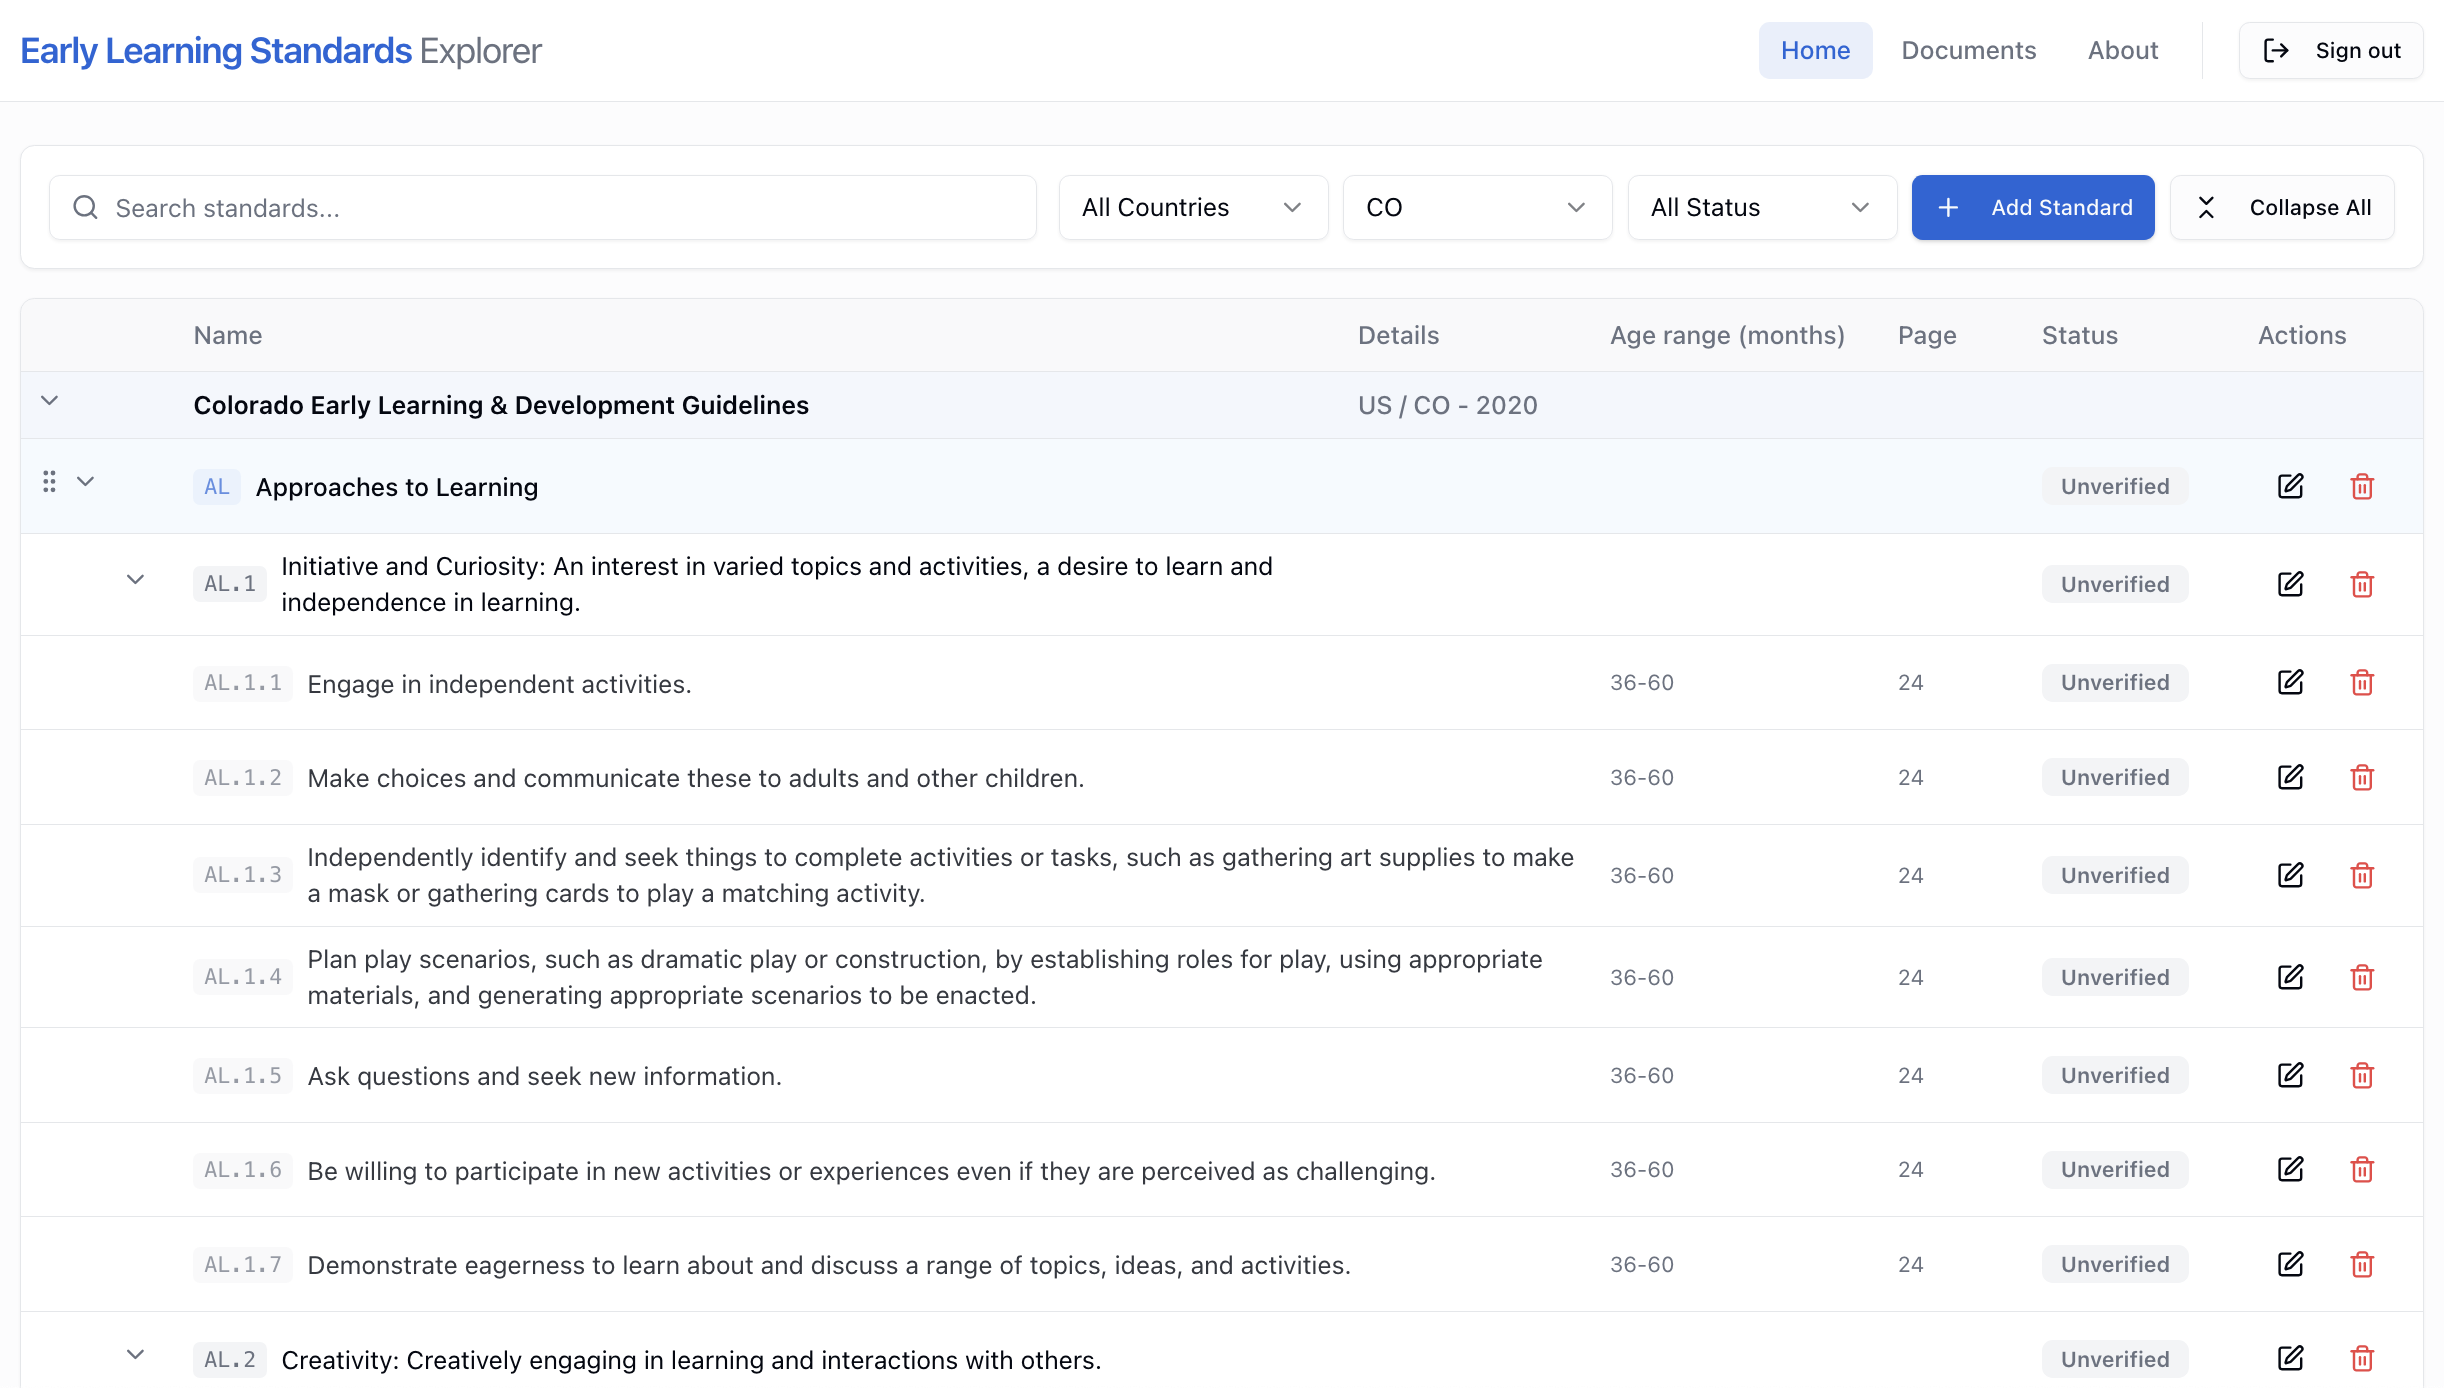
\includegraphics[width=\textwidth]{figures/colorado_els.png}
  \caption{The Standards Explorer, showing extracted Colorado standards resolved
  into the canonical schema of \S\ref{sec:schema}: domain \texttt{AL}, strand
  \texttt{AL.1}, and the indicators beneath it, each row carrying its age range
  and source page. The \emph{Status} column is the per-element human
  verification state of \S\ref{sec:method-confidence}, which is
  \textbf{independent of the model's confidence score}.}
  \label{fig:explorer}
\end{figure*}
